\PassOptionsToPackage{unicode=true}{hyperref} % options for packages loaded elsewhere
\PassOptionsToPackage{hyphens}{url}
%
\documentclass[ignorenonframetext,]{beamer}
\usepackage{pgfpages}
\setbeamertemplate{caption}[numbered]
\setbeamertemplate{caption label separator}{: }
\setbeamercolor{caption name}{fg=normal text.fg}
\beamertemplatenavigationsymbolsempty
% Prevent slide breaks in the middle of a paragraph:
\widowpenalties 1 10000
\raggedbottom
\setbeamertemplate{part page}{
\centering
\begin{beamercolorbox}[sep=16pt,center]{part title}
  \usebeamerfont{part title}\insertpart\par
\end{beamercolorbox}
}
\setbeamertemplate{section page}{
\centering
\begin{beamercolorbox}[sep=12pt,center]{part title}
  \usebeamerfont{section title}\insertsection\par
\end{beamercolorbox}
}
\setbeamertemplate{subsection page}{
\centering
\begin{beamercolorbox}[sep=8pt,center]{part title}
  \usebeamerfont{subsection title}\insertsubsection\par
\end{beamercolorbox}
}
\AtBeginPart{
  \frame{\partpage}
}
\AtBeginSection{
  \ifbibliography
  \else
    \frame{\sectionpage}
  \fi
}
\AtBeginSubsection{
  \frame{\subsectionpage}
}
\usepackage{lmodern}
\usepackage{amssymb,amsmath}
\usepackage{ifxetex,ifluatex}
\usepackage{fixltx2e} % provides \textsubscript
\ifnum 0\ifxetex 1\fi\ifluatex 1\fi=0 % if pdftex
  \usepackage[T1]{fontenc}
  \usepackage[utf8]{inputenc}
  \usepackage{textcomp} % provides euro and other symbols
\else % if luatex or xelatex
  \usepackage{unicode-math}
  \defaultfontfeatures{Ligatures=TeX,Scale=MatchLowercase}
\fi
% use upquote if available, for straight quotes in verbatim environments
\IfFileExists{upquote.sty}{\usepackage{upquote}}{}
% use microtype if available
\IfFileExists{microtype.sty}{%
\usepackage[]{microtype}
\UseMicrotypeSet[protrusion]{basicmath} % disable protrusion for tt fonts
}{}
\IfFileExists{parskip.sty}{%
\usepackage{parskip}
}{% else
\setlength{\parindent}{0pt}
\setlength{\parskip}{6pt plus 2pt minus 1pt}
}
\usepackage{hyperref}
\hypersetup{
            pdftitle={Neuroconductor: An R Platform for Medical Imaging Analysis},
            pdfauthor={John Muschelli http://johnmuschelli.com/ICSA\_2019.html  Johns Hopkins Bloomberg School of Public Health},
            pdfborder={0 0 0},
            breaklinks=true}
\urlstyle{same}  % don't use monospace font for urls
\newif\ifbibliography
\usepackage{color}
\usepackage{fancyvrb}
\newcommand{\VerbBar}{|}
\newcommand{\VERB}{\Verb[commandchars=\\\{\}]}
\DefineVerbatimEnvironment{Highlighting}{Verbatim}{commandchars=\\\{\}}
% Add ',fontsize=\small' for more characters per line
\usepackage{framed}
\definecolor{shadecolor}{RGB}{248,248,248}
\newenvironment{Shaded}{\begin{snugshade}}{\end{snugshade}}
\newcommand{\AlertTok}[1]{\textcolor[rgb]{0.94,0.16,0.16}{#1}}
\newcommand{\AnnotationTok}[1]{\textcolor[rgb]{0.56,0.35,0.01}{\textbf{\textit{#1}}}}
\newcommand{\AttributeTok}[1]{\textcolor[rgb]{0.77,0.63,0.00}{#1}}
\newcommand{\BaseNTok}[1]{\textcolor[rgb]{0.00,0.00,0.81}{#1}}
\newcommand{\BuiltInTok}[1]{#1}
\newcommand{\CharTok}[1]{\textcolor[rgb]{0.31,0.60,0.02}{#1}}
\newcommand{\CommentTok}[1]{\textcolor[rgb]{0.56,0.35,0.01}{\textit{#1}}}
\newcommand{\CommentVarTok}[1]{\textcolor[rgb]{0.56,0.35,0.01}{\textbf{\textit{#1}}}}
\newcommand{\ConstantTok}[1]{\textcolor[rgb]{0.00,0.00,0.00}{#1}}
\newcommand{\ControlFlowTok}[1]{\textcolor[rgb]{0.13,0.29,0.53}{\textbf{#1}}}
\newcommand{\DataTypeTok}[1]{\textcolor[rgb]{0.13,0.29,0.53}{#1}}
\newcommand{\DecValTok}[1]{\textcolor[rgb]{0.00,0.00,0.81}{#1}}
\newcommand{\DocumentationTok}[1]{\textcolor[rgb]{0.56,0.35,0.01}{\textbf{\textit{#1}}}}
\newcommand{\ErrorTok}[1]{\textcolor[rgb]{0.64,0.00,0.00}{\textbf{#1}}}
\newcommand{\ExtensionTok}[1]{#1}
\newcommand{\FloatTok}[1]{\textcolor[rgb]{0.00,0.00,0.81}{#1}}
\newcommand{\FunctionTok}[1]{\textcolor[rgb]{0.00,0.00,0.00}{#1}}
\newcommand{\ImportTok}[1]{#1}
\newcommand{\InformationTok}[1]{\textcolor[rgb]{0.56,0.35,0.01}{\textbf{\textit{#1}}}}
\newcommand{\KeywordTok}[1]{\textcolor[rgb]{0.13,0.29,0.53}{\textbf{#1}}}
\newcommand{\NormalTok}[1]{#1}
\newcommand{\OperatorTok}[1]{\textcolor[rgb]{0.81,0.36,0.00}{\textbf{#1}}}
\newcommand{\OtherTok}[1]{\textcolor[rgb]{0.56,0.35,0.01}{#1}}
\newcommand{\PreprocessorTok}[1]{\textcolor[rgb]{0.56,0.35,0.01}{\textit{#1}}}
\newcommand{\RegionMarkerTok}[1]{#1}
\newcommand{\SpecialCharTok}[1]{\textcolor[rgb]{0.00,0.00,0.00}{#1}}
\newcommand{\SpecialStringTok}[1]{\textcolor[rgb]{0.31,0.60,0.02}{#1}}
\newcommand{\StringTok}[1]{\textcolor[rgb]{0.31,0.60,0.02}{#1}}
\newcommand{\VariableTok}[1]{\textcolor[rgb]{0.00,0.00,0.00}{#1}}
\newcommand{\VerbatimStringTok}[1]{\textcolor[rgb]{0.31,0.60,0.02}{#1}}
\newcommand{\WarningTok}[1]{\textcolor[rgb]{0.56,0.35,0.01}{\textbf{\textit{#1}}}}
\usepackage{graphicx,grffile}
\makeatletter
\def\maxwidth{\ifdim\Gin@nat@width>\linewidth\linewidth\else\Gin@nat@width\fi}
\def\maxheight{\ifdim\Gin@nat@height>\textheight\textheight\else\Gin@nat@height\fi}
\makeatother
% Scale images if necessary, so that they will not overflow the page
% margins by default, and it is still possible to overwrite the defaults
% using explicit options in \includegraphics[width, height, ...]{}
\setkeys{Gin}{width=\maxwidth,height=\maxheight,keepaspectratio}
\setlength{\emergencystretch}{3em}  % prevent overfull lines
\providecommand{\tightlist}{%
  \setlength{\itemsep}{0pt}\setlength{\parskip}{0pt}}
\setcounter{secnumdepth}{0}

% set default figure placement to htbp
\makeatletter
\def\fps@figure{htbp}
\makeatother


\title{Neuroconductor: An R Platform for Medical Imaging Analysis}
\author{John Muschelli\url{http://johnmuschelli.com/ICSA_2019.html} Johns
Hopkins Bloomberg School of Public Health}
\date{}
\logo{
\includegraphics{bloomberg.logo.small.horizontal.blue.png}}

\begin{document}
\frame{\titlepage}

\begin{frame}

\end{frame}

\hypertarget{r-is-a-language-and-environment-for-statistical-computing-and-graphics.-httpscran.r-project.org}{%
\section{\texorpdfstring{R is a language and environment for
\textbf{statistical} computing and graphics.
\url{https://cran.r-project.org/}}{R is a language and environment  for statistical computing  and graphics.   https://cran.r-project.org/}}\label{r-is-a-language-and-environment-for-statistical-computing-and-graphics.-httpscran.r-project.org}}

\hypertarget{r-is-much-more-than-that-now-but}{%
\section{\texorpdfstring{R is \textbf{much more} than that now,
but\ldots{}}{R is much more than that now, but\ldots{}}}\label{r-is-much-more-than-that-now-but}}

\begin{frame}{What did R have for medical imaging?}
\protect\hypertarget{what-did-r-have-for-medical-imaging}{}

\url{https://imgflip.com/memegenerator/Grandma-Finds-The-Internet}

\end{frame}

\begin{frame}{What did R have for medical imaging?}
\protect\hypertarget{what-did-r-have-for-medical-imaging-1}{}

\end{frame}

\begin{frame}{What did R have for medical imaging?}
\protect\hypertarget{what-did-r-have-for-medical-imaging-2}{}

\end{frame}

\begin{frame}

\hypertarget{left_col2}{}
Workflow for an Analysis

\begin{itemize}
\tightlist
\item
  bash 
\item
  FSL 
\item
  ANTs 
\item
  MRIcroGL 
\item
  OsiriX 
\item
  SPM 12 
\end{itemize}

\hypertarget{right_col2}{}

\end{frame}

\begin{frame}

\hypertarget{left_col2}{}
Workflow for an Analysis

Multiple pieces of software used

\begin{itemize}
\tightlist
\item
  all different syntax
\end{itemize}

\hypertarget{right_col2}{}

\end{frame}

\begin{frame}[fragile]

\hypertarget{left_col2}{}
Our Goal:

Lower the bar to entry

\begin{itemize}
\tightlist
\item
  all ``one'' code (\texttt{R})

  \begin{itemize}
  \tightlist
  \item
    pipeline tool
  \item
    also ``native'' \texttt{R} code
  \end{itemize}
\end{itemize}

Complete pipeline

\begin{itemize}
\tightlist
\item
  preprocessing and analysis
\end{itemize}

\hypertarget{right_col2}{}

\end{frame}

\begin{frame}{Envy: Bioconductor }
\protect\hypertarget{envy-bioconductor}{}

\begin{itemize}
\tightlist
\item
  centralized bioinformatics packages (\textgreater{} 1300)
\item
  large community/developer team
\item
  published tutorials and workflows
\item
  additional requirements to CRAN (e.g.~packages need vignettes)
\end{itemize}

\end{frame}

\hypertarget{an-r-platform-for-medical-imaging-analysis}{%
\section{\texorpdfstring{ An R Platform for Medical Imaging
Analysis}{  An R Platform for   Medical Imaging Analysis}}\label{an-r-platform-for-medical-imaging-analysis}}

\begin{frame}{What is Neuroconductor?}
\protect\hypertarget{what-is-neuroconductor}{}

\begin{enumerate}
\tightlist
\item
  A centralized repository of packages (N = 97)
\item
  A community of developers (N = 26) and users
\item
  A website \url{https://neuroconductor.org/}.

  \begin{itemize}
  \tightlist
  \item
    with tutorials and help
  \end{itemize}
\item
  A team helping developers and users (John, Adi Gherman, Ciprian
  Crainiceanu, Brian Caffo)
\end{enumerate}

\end{frame}

\begin{frame}[fragile]{Benefits of Neuroconductor}
\protect\hypertarget{benefits-of-neuroconductor}{}

Allow imaging to use all \texttt{R} has to offer:

\begin{itemize}
\tightlist
\item
  Statistics and Machine Learning (\texttt{tensorflow})
\item
  Versioning and testing (\texttt{GitHub})
\item
  Reproducible reports and analyses
\item
  Shiny (web applications)
\item
  Genomics/Imaging analysis in one platform

  \begin{itemize}
  \tightlist
  \item
    Bioconductor
  \end{itemize}
\end{itemize}

\end{frame}

\begin{frame}{Goal: Centralize the packages (currently 97)}
\protect\hypertarget{goal-centralize-the-packages-currently-97}{}

\end{frame}

\begin{frame}{New release (December 2019)}
\protect\hypertarget{new-release-december-2019}{}

\begin{center}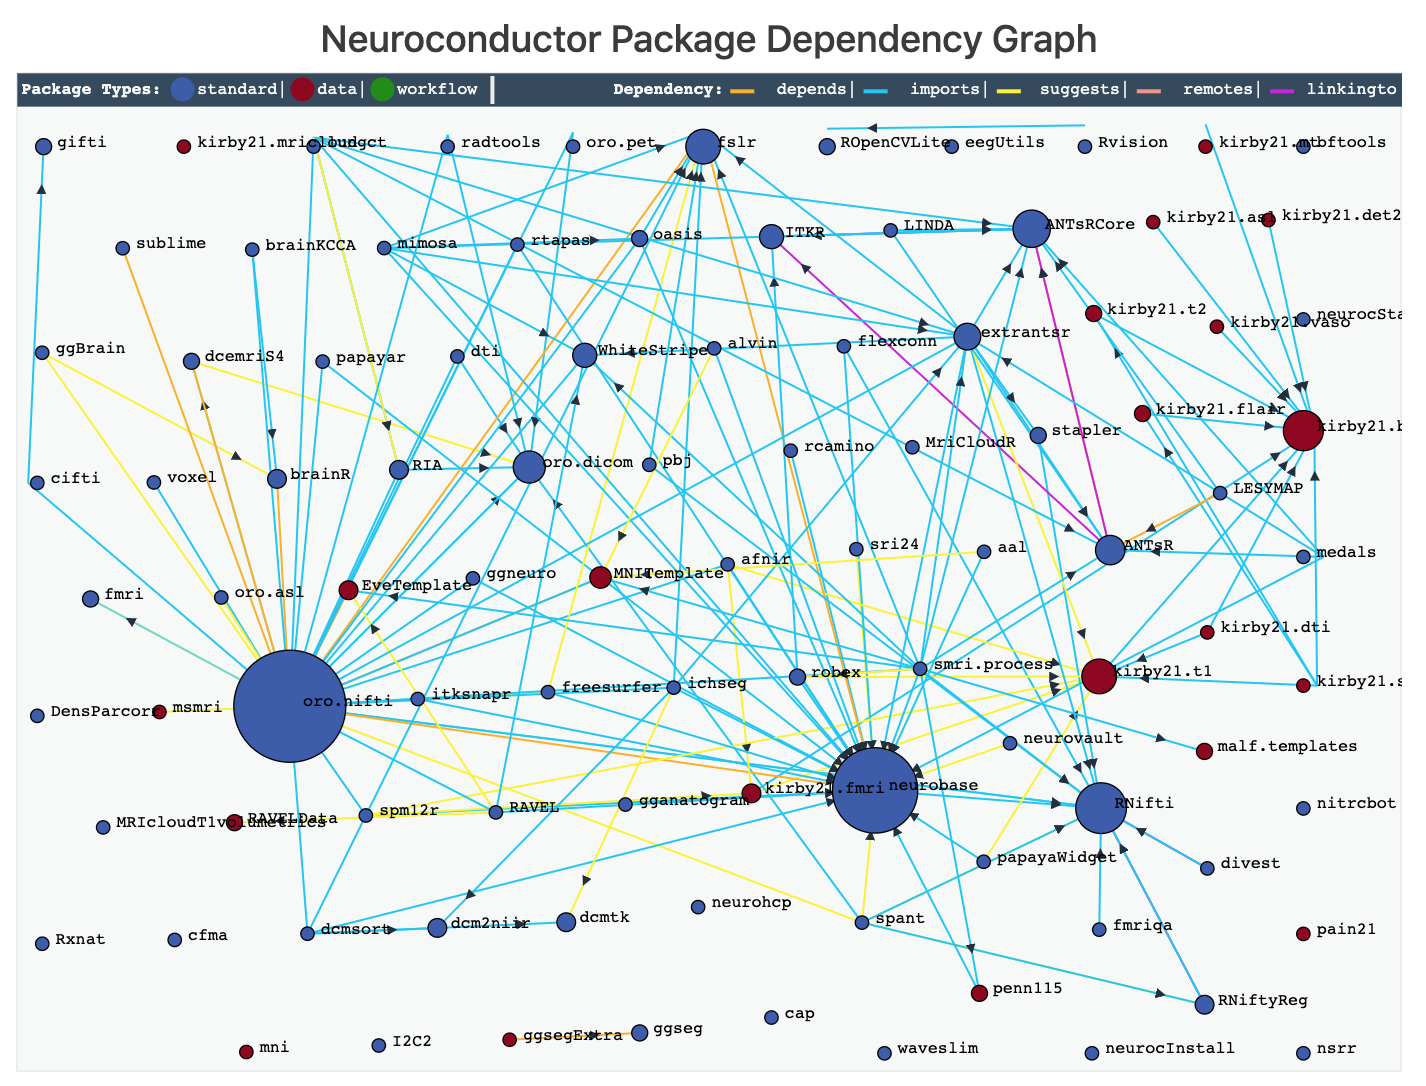
\includegraphics[width=0.7\linewidth]{figures/dependency_graph} \end{center}

\end{frame}

\begin{frame}[fragile]{Using R as a Pipeline Tool: fslr }
\protect\hypertarget{using-r-as-a-pipeline-tool-fslr}{}

\begin{itemize}
\tightlist
\item
  \texttt{fslr} - call FSL from R (requires FSL)
\end{itemize}

\end{frame}

\begin{frame}[fragile]{ichseg: ICH Segmentation of CT images }
\protect\hypertarget{ichseg-ich-segmentation-of-ct-images}{}

\begin{Shaded}
\begin{Highlighting}[]
\NormalTok{ichseg}\OperatorTok{::}\KeywordTok{ich_segment}\NormalTok{(}\DataTypeTok{img =} \StringTok{"/path/to/ct/scan"}\NormalTok{)}
\end{Highlighting}
\end{Shaded}

\begin{center}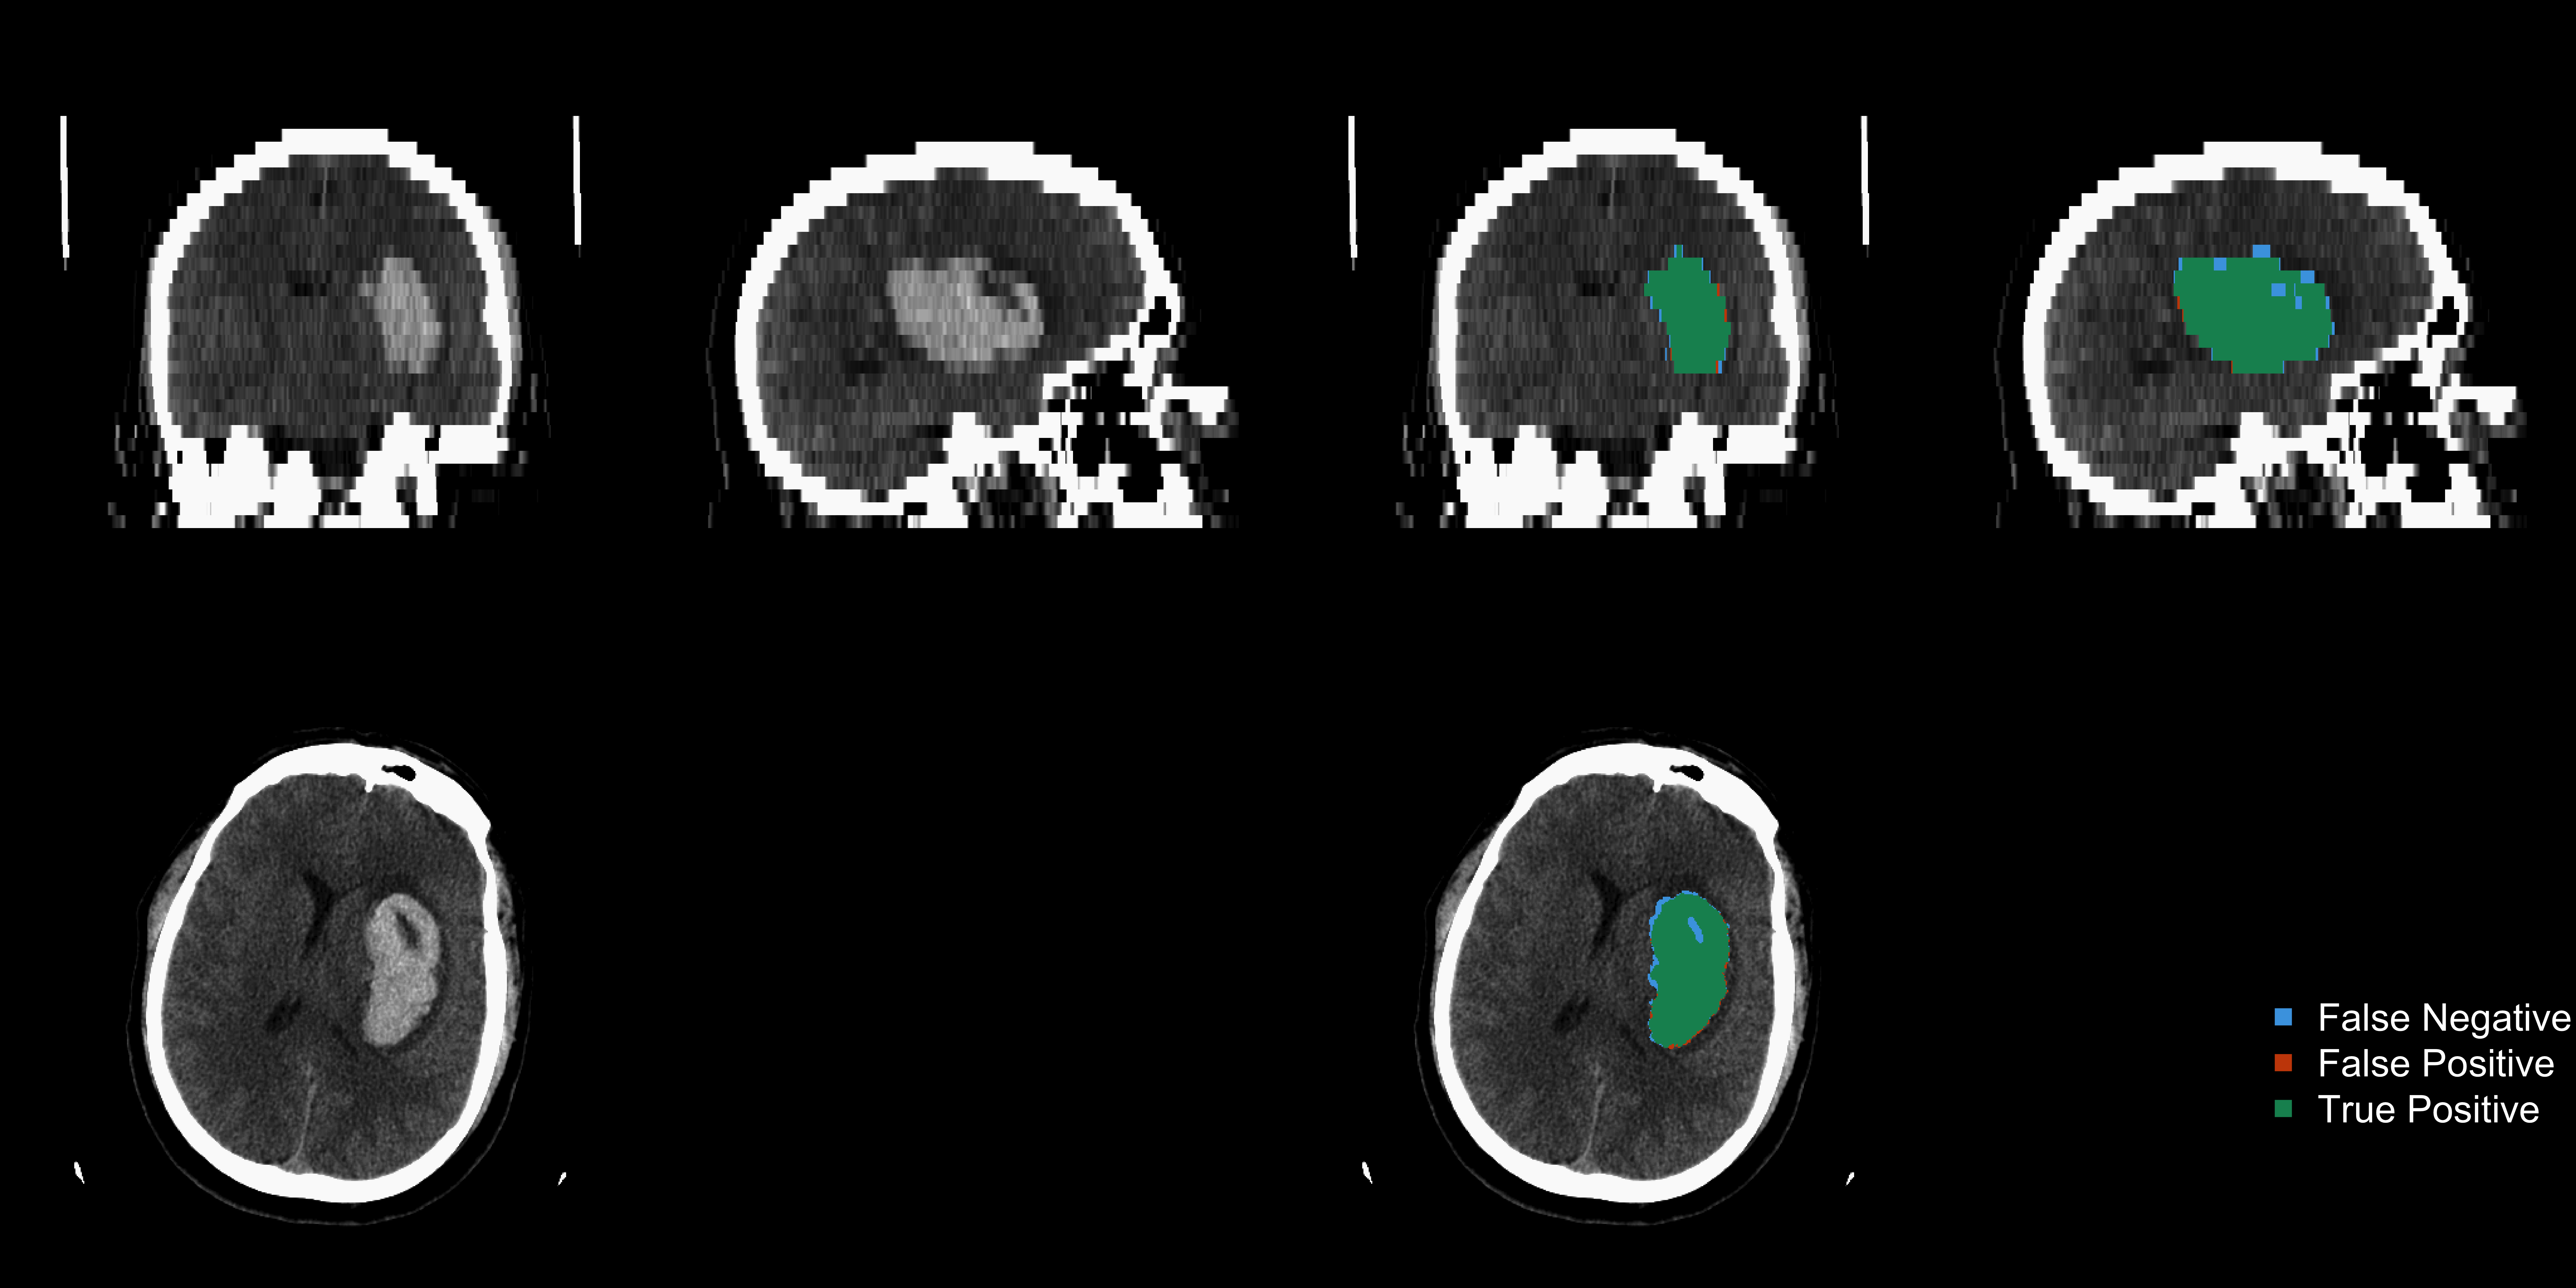
\includegraphics[width=0.85\linewidth]{figures/ichseg_example} \end{center}

\end{frame}

\begin{frame}{lungct: Analysis of Lung CT Scans }
\protect\hypertarget{lungct-analysis-of-lung-ct-scans}{}

\begin{center}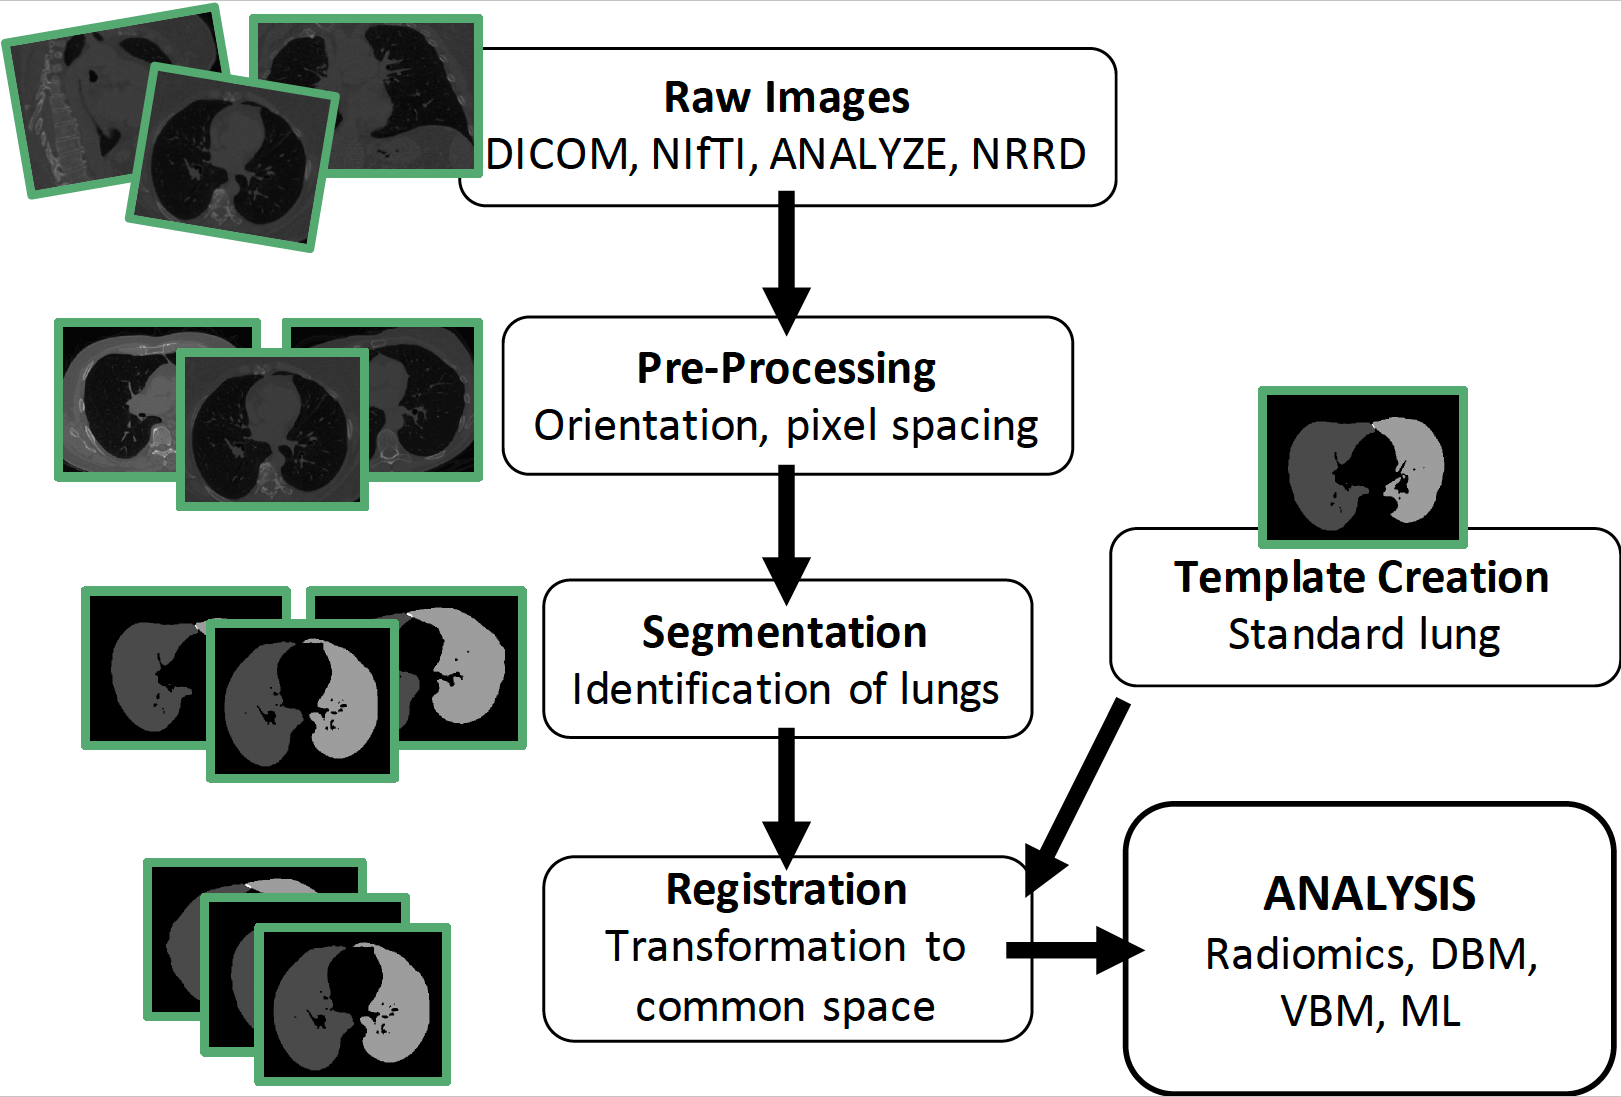
\includegraphics[width=0.75\linewidth]{figures/lungct_pipeline} \end{center}

\end{frame}

\begin{frame}

\hypertarget{left_col2}{}
Development Pipeline:

Check the package for stability

\begin{itemize}
\tightlist
\item
  check against other imaging software (e.g.~FSL)
\end{itemize}

\hypertarget{right_col2}{}

\end{frame}

\begin{frame}

\hypertarget{left_col2}{}
Neuroconductor Goal:

Detailed \textbf{tutorials} on how to actually perform an analysis

\hypertarget{right_col2}{}
From \url{http://i.imgur.com/0Y1xISa.gifv}.

\url{http://johnmuschelli.com/neuroc}

\end{frame}

\begin{frame}{Some (Unpopular) Opinions}
\protect\hypertarget{some-unpopular-opinions}{}

\begin{enumerate}
\tightlist
\item
  No code = no method. ``Available upon request'' - not great
\item
  We are not the leaders in imaging
\item
  Not everyone cares about our methods
\item
  Many engineers are better in imaging at a) distributing code and b)
  selling their method
\end{enumerate}

\end{frame}

\begin{frame}{Helping Developers}
\protect\hypertarget{helping-developers}{}

\hypertarget{left_col}{}
\begin{itemize}
\tightlist
\item
  GitHub allows the Neuroconductor team to help fix issues
\item
  Pull Requests to developers
\item
  Standardized checking of Packages (Travis configuration)
\item
  Remove unnecessary hurdles for developers
\end{itemize}

\hypertarget{right_col}{}

Image from:
\url{https://giphy.com/gifs/medblr-medschool-dr-dres-anatomy-uRb2p09vY8lEs}

\end{frame}

\begin{frame}{Questions?}
\protect\hypertarget{questions}{}

Email:

\end{frame}

\begin{frame}{Training we are providing}
\protect\hypertarget{training-we-are-providing}{}

Coursera Course: Introduction to Neurohacking In R

 \url{https://www.coursera.org/learn/neurohacking/}

\url{http://johnmuschelli.com/imaging_in_r/}

\end{frame}

\begin{frame}{RNifti and RNiftyReg}
\protect\hypertarget{rnifti-and-rniftyreg}{}

\begin{itemize}
\tightlist
\item
  provides lightweight objects as C++ pointers (fast operations)
\item
  Registration of Images
\item
  Wrapped in Rcpp: Works on all platforms
\end{itemize}

\end{frame}

\begin{frame}{ANTsR}
\protect\hypertarget{antsr}{}

Based on ANTs: Advanced Normalization Tools

\begin{itemize}
\tightlist
\item
  State-of-the-art image processing pipelines
\item
  Built at UPenn under Brian Avants

  \begin{itemize}
  \tightlist
  \item
    Group has won challenges for imaging analysis
  \end{itemize}
\item
  Still actively maintained and developed
\item
  Depends on the Insight ToolKit (ITK) medical image processing library
\end{itemize}

\end{frame}

\begin{frame}{neurohcp: Human Connectome Project}
\protect\hypertarget{neurohcp-human-connectome-project}{}

\begin{itemize}
\tightlist
\item
  Allows you to download data from
  \href{https://www.humanconnectome.org/}{Human Connectome Project}
\item
  The 1200 Subjects release: behavioral and 3T MR imaging data from 1206
  healthy young adult participants. Standardized protocol.
\item
  Tutorial: \url{http://johnmuschelli.com/neuroc/neurohcp}
\end{itemize}

\end{frame}

\begin{frame}{rcamino: Port of Camino Software}
\protect\hypertarget{rcamino-port-of-camino-software}{}

\begin{itemize}
\tightlist
\item
  Wraps \href{http://camino.cs.ucl.ac.uk/}{Camino Diffusion MRI Toolkit}
\item
  Takes in b-values, b-vectors, and tensors
\item
  Fits models for DTI data
\item
  \url{http://johnmuschelli.com/neuroc/DTI_analysis_rcamino/index.html}
\end{itemize}

\end{frame}

\begin{frame}{malf.templates: Segmented T1-weighted Images}
\protect\hypertarget{malf.templates-segmented-t1-weighted-images}{}

\begin{itemize}
\tightlist
\item
  Data from the MICCAI 2012 Challenge on Multi-atlas Labelling Data
\item
  From OASIS project and the labeled data as provided by
  Neuromorphometrics, Inc.~(\url{http://Neuromorphometrics.com/})
\end{itemize}

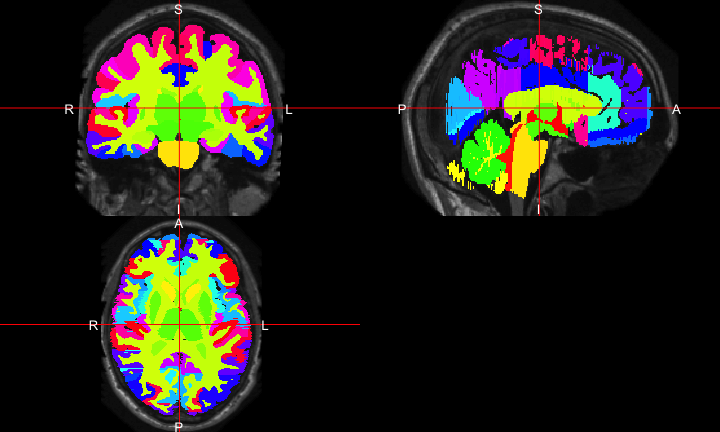
\includegraphics{ICSA_2019_files/figure-beamer/unnamed-chunk-6-1.pdf}

\end{frame}

\begin{frame}{MALF: Skull Stripping Example}
\protect\hypertarget{malf-skull-stripping-example}{}

From (Doshi et al. 2013):

\begin{itemize}
\tightlist
\item
  Register templates to an subject T1
\item
  Apply transformation to the label/mask, average over voxels

  \begin{itemize}
  \tightlist
  \item
    there are ``smarter'' (e.g.~weighted) ways
  \end{itemize}
\end{itemize}

\hypertarget{refs}{}
\leavevmode\hypertarget{ref-mass}{}%
Doshi, Jimit, Guray Erus, Yangming Ou, Bilwaj Gaonkar, and Christos
Davatzikos. 2013. ``Multi-Atlas Skull-Stripping.'' \emph{Academic
Radiology} 20 (12): 1566--76.

\end{frame}

\end{document}
